\documentclass[12pt,oneside]{book} 

% Cargamos toda la configuración y paquetes
% ======================================================================
% PREÁMBULO: Tesina de Licenciatura - Configuración Unificada
% ======================================================================

% --------------------------------------------------
% 1. Codificación, Fuentes e Idioma
% --------------------------------------------------
\usepackage[utf8]{inputenc}
\usepackage[T1]{fontenc}
\usepackage[spanish,es-tabla]{babel}

% Tipografía formal Times New Roman estándar
\usepackage{mathptmx}

% --------------------------------------------------
% 1.1. Color Institucional y Fondos de Portada (DEPENDENCIAS DE PORTADA)
% --------------------------------------------------
\usepackage[dvipsnames]{xcolor}
\definecolor{AzulBUAP}{RGB}{0, 50, 110} % Azul oficial BUAP[cite: 4]
\usepackage{eso-pic}                     % Permite colocar marcas de agua y líneas de fondo[cite: 4]

% --------------------------------------------------
% 2. Bibliografía APA 7 (BibLaTeX + Biber)
% --------------------------------------------------
\usepackage{csquotes}
\usepackage[
  backend=biber,
  style=apa,
  language=spanish
]{biblatex}
\addbibresource{referencias.bib}

% --------------------------------------------------
% 3. Geometría de Página
% --------------------------------------------------
\usepackage[
  letterpaper,
  margin=2.54cm,
  headheight=15pt,
  headsep=12pt
]{geometry}

% --------------------------------------------------
% 4. Formato de Párrafo e Interlineado
% --------------------------------------------------
\usepackage{setspace}
\doublespacing                         % Interlineado doble APA 7
\setlength{\parindent}{1.27cm}         % Sangría de primera línea uniforme
\setlength{\parskip}{0pt}
\setcounter{secnumdepth}{4}

% --------------------------------------------------
% 5. Formato de Títulos (APA 7)
% --------------------------------------------------
\usepackage{titlesec}
\titleformat{\chapter}[display]
  {\normalfont\huge\bfseries\centering}
  {\chaptertitlename\ \thechapter}
  {10pt}
  {\Huge}
\titlespacing*{\chapter}{0pt}{10pt}{25pt}

\titleformat{\section}
  {\normalfont\Large\bfseries}
  {\thesection}
  {1em}
  {}
\titlespacing*{\section}{0pt}{15pt}{8pt}

\titleformat{\subsection}
  {\normalfont\large\bfseries\itshape}
  {\thesubsection}
  {1em}
  {}

% --------------------------------------------------
% 6. Control de Encabezados y Foliación Uniforme
% --------------------------------------------------
\usepackage{emptypage}
\usepackage{fancyhdr}

\pagestyle{fancy}
\fancyhf{}
\renewcommand{\headrulewidth}{0pt}
\rhead{\thepage} % Número siempre fijo en la esquina superior derecha

\fancypagestyle{plain}{%
  \fancyhf{}%
  \renewcommand{\headrulewidth}{0pt}%
  \rhead{\thepage}%
}

% --------------------------------------------------
% 7. Tablas, Flotantes y Figuras
% --------------------------------------------------
\usepackage{booktabs}
\usepackage{longtable}
\usepackage{multirow}
\usepackage{graphicx}
\usepackage{float}
\usepackage{array}       
\usepackage{amsmath,amssymb,amsthm}
\newtheorem{theorem}{Teorema}[chapter]

\usepackage{caption}
\captionsetup{
  justification=raggedright,
  singlelinecheck=false,
  labelfont=bf,
  font=small
}
\usepackage{subcaption}

% --------------------------------------------------
% 8. Hipervínculos Compatibles con APA 7
% --------------------------------------------------
\usepackage[hidelinks]{hyperref}

% Permite que el enlace funcione sin romper la estructura de los paréntesis
\DeclareFieldFormat{citehyperref}{%
  \iffieldundef{postnote}
    {\bibhyperref{#1}}
    {\bibhyperref{#1}}}

\begin{document}

\frontmatter

% 1. Portada Institucional
\begin{titlepage}
\thispagestyle{empty}

% ==========================================
% FONDO (Logo y líneas)
% ==========================================
\AddToShipoutPictureBG*{%
  \AtPageLowerLeft{%
    % 1. EL LOGO
    \put(1cm, 22cm){%
      
\includegraphics[width=5cm, keepaspectratio]{assets/img/logos/BUAP.png}%
    }%

    % 2. LÍNEAS HORIZONTALES
    \put(7cm, 24.5cm){\color{AzulBUAP}\rule{12.5cm}{4pt}}%
    \put(6.5cm, 24.2cm){\color{AzulBUAP}\rule{13cm}{0.8pt}}%

    % 3. LÍNEAS VERTICALES
    \put(3cm, 4.1cm){\color{AzulBUAP}\rule{1pt}{17.5cm}}%
    \put(3.35cm, 2.1cm){\color{AzulBUAP}\rule{4pt}{19.5cm}}%
    \put(3.75cm, 3.1cm){\color{AzulBUAP}\rule{1pt}{18.5cm}}%
  }%
}

% ==========================================
% TEXTO DE LA PORTADA
% ==========================================
\vspace*{-1.8cm}
\hfill
\begin{minipage}[t]{12.5cm}
  \centering
  
  {\bfseries\Large BENEMÉRITA UNIVERSIDAD\\[0.15cm] AUTÓNOMA DE PUEBLA}
  
  \vspace{1.2cm}
  
  {\bfseries\large FACULTAD DE CIENCIAS DE LA COMPUTACIÓN}\\[0.15cm]
  
  \vspace{1.5cm}
  
  {\bfseries\LARGE ``PLATAFORMA WEB PARA EL SEGUIMIENTO DE TESIS, ASESORÍAS Y ACTIVIDADES DE POSGRADO''}
  
  \vspace{1.0cm}
  
  {\bfseries\Large TESINA}\\[0.75cm]
  {\normalsize QUE PARA OBTENER EL TÍTULO DE:}\\[0.25cm]
  {\bfseries\large LICENCIADO EN CIENCIAS DE LA COMPUTACIÓN}
  
  \vspace{1.0cm}
  
  {\normalsize PRESENTA:}\\[0.2cm]
  {\bfseries\large LUIS FRANCISCO MATLALCUATZI GONZÁLEZ}\\[0.15cm]
  {\normalsize Matrícula: 201743936}
  
  \vspace{1.0cm}
  
  {\normalsize DIRECTOR DE TESINA:}\\[0.2cm]
  {\bfseries\large DR. JUAN MANUEL GONZÁLEZ CALLEROS}
  
  \vspace{1.5cm}
  
  {\bfseries CIUDAD UNIVERSITARIA, PUEBLA, PUE.}\\[0.15cm]
  {\normalsize Septiembre de 2026}
\end{minipage}

\end{titlepage}
\cleardoublepage

% 2. Constancia de Visto Bueno (cuando la tengas en su archivo)
% \input{constancia_vobo.tex}
% \cleardoublepage

\tableofcontents        % Índice General
\cleardoublepage
\listoftables           % Índice de Tablas
\cleardoublepage
\listoffigures          % Índice de Figuras
\cleardoublepage

% ======================================================================
% CUERPO DE LA TESINA (Inicia numeración arábiga continua: 1, 2, 3...)
% ======================================================================
\mainmatter 

% Capítulo 1: Introducción
\chapter{Introducción}
\label{cap:introduccion}

En los programas de posgrado universitario, la elaboración de la tesis constituye una de las etapas académicas más determinantes para la formación de los estudiantes, donde la comunicación continua y el acompañamiento con el asesor son fundamentales para evitar que los alumnos se atrasen. Sin embargo, este proceso suele verse afectado por el uso de herramientas informales de comunicación, tales como correos electrónicos personales y aplicaciones de mensajería. Esta práctica habitual provoca la pérdida de archivos, confusiones entre las distintas versiones de un mismo documento y el olvido frecuente de los acuerdos tomados en las asesorías debido a la falta de minutas organizadas. A su vez, los sistemas informáticos que ya tiene la universidad se concentran casi en su totalidad en trámites administrativos generales (como inscripciones y control escolar), sin contar con apartados específicos para dar seguimiento al trabajo continuo de la tesis ni avisar a tiempo a las coordinaciones cuando un alumno pasa mucho tiempo inactivo.

Para dar una respuesta a esta problemática, en este trabajo se propone el diseño y desarrollo de una página web orientada a reunir y organizar el seguimiento de las actividades de tesis. Con el fin de asegurar que el proyecto se termine dentro de los tiempos fijados para la tesina, el alcance de esta primera versión funcional se delimita a tres funciones esenciales: Recepción y consulta de entregables en formato PDF, Registro digital de minutas, Supervisión de fechas y control de inactividad. 

% =========================================================================
% LLAMADA A LAS SECCIONES HIJAS CON SALTO DE PÁGINA
% =========================================================================

\clearpage
\section{Resumen}\label{sec:resumen}El presente proyecto consiste en el diseño y desarrollo de una \textbf{página web} orientada a facilitar el seguimiento, control y organización de las actividades de tesis en programas de posgrado. El alcance de esta primera versión del sistema se delimita a tres funciones esenciales: la recepción y consulta de avances en formato PDF guardando el historial de cambios sin sobreescribir archivos; el registro digital de minutas al término de cada asesoría con los acuerdos y tareas establecidos; y la revisión básica de fechas para identificar y avisar oportunamente cuando un alumno sume más de 30 días de inactividad académica. La propuesta reúne estas herramientas en un solo lugar de manera accesible y segura para alumnos, asesores y coordinadores, sentando las bases operativas del acompañamiento académico para evitar atrasos en la titulación de los tesistas.  \vspace{0.5cm}

\noindent \textbf{Palabras clave:} seguimiento de tesis, apoyo escolar, control de archivos, minutas de asesoría, página web educativa, prevención del rezago
\clearpage
\section{Objetivos del Proyecto}
\label{sec:objetivos}

\subsection{Objetivo General}
\label{subsec:obj_general}
    Desarrollar una primera versión de una \textbf{página web} para organizar, centralizar y dar seguimiento continuo a las actividades de tesis en los programas de posgrado, reuniendo en un solo lugar las herramientas necesarias para que alumnos, asesores y coordinadores trabajen de forma coordinada. 

    Para lograr esto, la página web se enfocará en resolver tres necesidades principales:

    \textbf{Control de documentos:} Permitir que los estudiantes suban sus borradores de tesis exclusivamente en formato PDF, guardando un historial ordenado de cada versión entregada para que el asesor pueda revisarlas sin riesgo de sobreescribir correcciones anteriores ni borrar archivos por error.

    \textbf{Registro de asesorías:} Facilitar el llenado y la consulta de minutas digitales al terminar cada sesión de trabajo, dejando por escrito la fecha, los temas tratados y la lista de acuerdos o tareas pendientes que deben cumplir tanto el alumno como el profesor.

    \textbf{Supervisión y prevención del rezago:} Llevar un control automático de las fechas para detectar si un estudiante acumula más de 30 días sin registrar avances o reuniones, mostrando avisos claros para que la coordinación y los tutores puedan intervenir a tiempo y evitar que los alumnos se atrasen en su titulación.
\subsection{Objetivos Específicos}
\label{subsec:obj_especificos}

Para cumplir con el objetivo general, el proyecto se divide en las siguientes etapas y actividades específicas:

\begin{enumerate}
    \item \textbf{Diseño de accesos y pantallas según el tipo de usuario (Roles):}
    \begin{itemize}
        \item Diseñar pantallas sencillas, claras y fáciles de usar para que cualquier persona pueda navegar sin perderse.
        \item Separar el acceso en tres tipos de cuentas: el estudiante (para subir sus trabajos y revisar tareas), el asesor (para dejar comentarios y calificar acuerdos) y la coordinación (para ver el estado general de todos los alumnos).
        \item \textit{Restricción:} Por seguridad y privacidad, cada usuario solo podrá ver su propia información; ningún estudiante podrá ver los archivos o minutas de otro compañero.
    \end{itemize}

    \item \textbf{Módulo de entrega y control de documentos de tesis:}
    \begin{itemize}
        \item Permitir que el alumno suba sus entregas a la plataforma para que el profesor las pueda consultar y descargar cuando las vaya a revisar.
        \item Llevar un registro ordenado que guarde cada versión del documento con su fecha y hora, mostrando un historial claro de los cambios realizados.
        \item \textit{Restricciones:} 
        \begin{itemize}
            \item El sistema solo aceptará archivos en formato PDF para asegurar que el contenido no se desacomode ni se altere.
            \item Queda prohibido sobreescribir o borrar versiones anteriores; cada nuevo documento se guardará como una versión adicional (por ejemplo: Versión 1, Versión 2) para conservar el historial completo.
        \end{itemize}
    \end{itemize}

    \item \textbf{Módulo para el registro y consulta de minutas de asesoría:}
    \begin{itemize}
        \item Crear un formulario digital donde el asesor o el alumno puedan registrar rápidamente lo sucedido al terminar cada sesión de trabajo.
        \item Dejar por escrito los temas que se revisaron, la fecha de la reunión y la lista de acuerdos o tareas pendientes para la siguiente cita.
        \item \textit{Restricciones:} Toda minuta debe incluir obligatoriamente la fecha de la sesión y al menos un acuerdo o compromiso registrado para poder ser guardada en la página web.
    \end{itemize}

    \item \textbf{Módulo de fechas y avisos de inactividad para evitar atrasos:}
    \begin{itemize}
        \item Monitorear las fechas del sistema calculando de forma automática los días transcurridos desde la última entrega de borrador o desde la última minuta registrada.
        \item Mostrar avisos visuales claros a los tutores y a la coordinación cuando un estudiante lleve mucho tiempo sin interactuar en el sistema.
        \item \textit{Restricción:} El sistema marcará un aviso de inactividad únicamente cuando el alumno acumule más de 30 días consecutivos sin subir un avance ni registrar una minuta de asesoría.
    \end{itemize}

    \item \textbf{Pruebas de funcionamiento del sistema:}
    \begin{itemize}
        \item Probar individualmente cada parte de la página web (subida de archivos, llenado de minutas y cálculo de días) para verificar que funcionen sin errores.
        \item Confirmar con ejemplos reales que los archivos se descarguen bien, que las cuentas respeten sus permisos y que las alertas se activen en las fechas correctas.
    \end{itemize}
\end{enumerate}
\section{Justificación}
\label{sec:justificacion}

La elaboración de una tesis de posgrado requiere una comunicación constante entre el estudiante y su asesor. Sin embargo, en la práctica diaria este proceso suele llevarse a cabo por medios informales como aplicaciones de mensajería instantánea y correos electrónicos personales. Aunque estas herramientas son de uso común, no fueron diseñadas para la gestión académica. Como resultado, los borradores se mezclan entre tantos mensajes, se borran archivos por error, no se sabe con certeza cuál es la versión más reciente del trabajo y se olvidan las tareas acordadas porque no existe un registro formal de las reuniones.

A su vez, los sistemas informáticos con los que cuenta la institución se enfocan casi por completo en trámites escolares generales (como inscripciones y calificaciones), dejando sin apoyo el seguimiento continuo del trabajo de investigación. Por esta razón, se justifica el diseño y desarrollo de una \textbf{página web} que concentre en un solo lugar digital todo el proceso de asesorías, resolviendo de manera directa las necesidades de cada participante:

\begin{enumerate}
    \item \textbf{Beneficio para los estudiantes:} Les proporciona un espacio seguro donde subir sus avances de tesis en formato PDF, con la tranquilidad de que sus entregas anteriores quedan guardadas en un historial y no se van a perder ni sobreescribir. Además, les permite revisar en cualquier momento las minutas con los compromisos y fechas límite acordados con su profesor.
    
    \item \textbf{Beneficio para los asesores:} Les facilita revisar los documentos ordenadamente por versiones, retroalimentar el trabajo y registrar en pocos minutos los acuerdos al término de cada sesión, evitando confusiones y malos entendidos sobre las tareas pendientes.
    
    \item \textbf{Beneficio para la coordinación de posgrado:} Le permite saber el estado real del avance de los estudiantes sin tener que pedir reportes manuales a cada maestro. Gracias al control de fechas, la coordinación puede identificar de inmediato qué alumnos tienen más de 30 días de inactividad, pudiendo intervenir a tiempo para evitar que abandonen la tesis o se atrasen en su titulación.
\end{enumerate}

Por último, delimitar el alcance a una primera versión centrada en tres funciones básicas (control de archivos PDF sin sobreescritura, minutas digitales y alertas por inactividad mayor a 30 días) garantiza la viabilidad del proyecto. Esto permite concluir el sistema dentro de los tiempos estipulados para la tesina, entregando una herramienta funcional, fácil de utilizar y útil para la facultad, sobre la cual se podrán agregar más funciones en desarrollos futuros.
% Capítulo 2: Marco Teórico y Estado del Arte
\chapter{Marco teórico y estado del arte}
\label{cap:marco_teorico_estado_arte}

En este capítulo se presentan dos partes fundamentales para respaldar el desarrollo de la página web. En la primera parte, correspondiente al estado del arte, se analizan los estudios científicos y las plataformas existentes en el mercado para identificar qué funciones ofrecen y qué limitaciones presentan en el seguimiento de tesis. En la segunda parte, correspondiente al marco teórico, se explican los conceptos escolares del proceso de titulación y los fundamentos técnicos de software indispensables para comprender el funcionamiento y la estructura del sistema propuesto.

% Inclusión de las dos grandes divisiones del capítulo
\section{Estado del arte}
\label{sec:estado_arte}

% Llamada a las subsecciones del estado del arte
\subsection{Introducción al estado del arte}
\label{subsec:intro_estado_arte}

Antes de construir una nueva herramienta informática, resulta indispensable conocer qué soluciones han propuesto otros investigadores y qué aplicaciones se utilizan actualmente en las universidades para atender el seguimiento de tesis. 

Analizar estos antecedentes permite identificar qué aciertos han tenido otros proyectos y qué fallas o vacíos operativos continúan presentes. De esta manera, el diseño de la página web no parte desde cero ni repite errores comunes, sino que se orienta de forma directa a resolver los problemas reales que enfrentan los estudiantes, asesores y coordinadores en la entrega de borradores, la organización de reuniones y el control de tiempos.
\subsection{Revisión de investigaciones científicas similares}
\label{subsec:investigaciones_cientificas}

Varios investigadores han diseñado páginas web y sistemas digitales para evitar que los estudiantes se atrasen al realizar su tesis de posgrado y para que la comunicación con sus asesores sea más ordenada.

En primer lugar, \textcite{sim2023technology} explican que cuando las asesorías se dan solo por medios informales como WhatsApp o correos personales, los acuerdos y tareas se olvidan con facilidad. Por esta razón, afirman que una plataforma web ayuda a mantener un contacto continuo y organizado entre ambas partes.

Por otra parte, \textcite{ali2024thesis} desarrollaron un sistema web para registrar los temas de tesis y ordenar las entregas de avances de los estudiantes. Su investigación demostró que reunir todos los archivos en un solo lugar digital evita que los trabajos se extravíen en correos o memorias USB.

De igual manera, \textcite{sayeh2021web} puso a prueba una página web para supervisar los avances de tesis en una facultad de computación. Su trabajo confirmó que registrar de forma ordenada cada borrador entregado permite que los profesores conozcan el avance real de cada tesista sin necesidad de imprimir hojas de papel.

En cuanto al cuidado de los documentos, \textcite{mebtouche2025national} señala que las universidades requieren plataformas digitales seguras para resguardar los archivos de las investigaciones, evitando que los trabajos se borren o se pierdan con el paso de los años.

Por último, \textcite{lando2025digital} analizaron diversas plataformas de posgrado y encontraron que muchos alumnos abandonan la tesis porque el sistema no cuenta con avisos de tiempo. Si un estudiante pasa varias semanas sin entregar nada y nadie se entera a tiempo, es muy probable que termine desertando del programa.

En la Tabla \ref{tab:literatura_cientifica} se comparan estas investigaciones señalando qué aporta cada una y qué funciones faltaron por resolver frente a lo que propone este proyecto.

\begin{table}[!ht]
\centering
\small
\singlespacing
\caption{Comparación de investigaciones científicas analizadas.}
\label{tab:literatura_cientifica}
\begin{tabular}{
  p{\dimexpr 0.22\linewidth - 2\tabcolsep\relax}
  p{\dimexpr 0.24\linewidth - 2\tabcolsep\relax}
  p{\dimexpr 0.26\linewidth - 2\tabcolsep\relax}
  p{\dimexpr 0.20\linewidth - 2\tabcolsep\relax}
}
\toprule
\textbf{Investigación} & \textbf{¿Qué propone?} & \textbf{Aporte importante} & \textbf{¿Qué le faltó resolver?} \\
\midrule
\textcite{sim2023technology} & 
Uso de páginas web para asesorías. & 
Demuestra que el contacto continuo evita que el alumno se quede rezagado. & 
No define reglas para guardar versiones sin sobreescribir archivos. \\
\addlinespace
\textcite{ali2024thesis} & 
Página web para registrar temas de tesis. & 
Reúne los borradores y proyectos en un solo lugar digital. & 
No incluye un apartado para registrar minutas de acuerdos. \\
\addlinespace
\textcite{sayeh2021web} & 
Sistema de seguimiento en computación. & 
Permite revisar el avance de tesis sin requerir hojas de papel. & 
No cuenta con un reloj automático que mande alertas de inactividad. \\
\addlinespace
\textcite{mebtouche2025national} & 
Plataforma escolar para resguardar tesis. & 
Organiza y protege los documentos finales para que no se pierdan. & 
Solo guarda tesis concluidas; no ayuda en las revisiones del día a día. \\
\addlinespace
\textcite{lando2025digital} & 
Estudio sobre herramientas de asesoría. & 
Comprueba que la falta de avisos de tiempo causa el abandono escolar. & 
Es un artículo de análisis teórico, no crearon el software. \\
\bottomrule
\end{tabular}
\end{table}
\subsection{Comparación con programas y plataformas existentes (Benchmark)}
\label{subsec:benchmark}

En las escuelas e instituciones de trabajo ya se utilizan diversas herramientas digitales para coordinar actividades, enviar tareas o compartir archivos; sin embargo, ninguna de ellas fue pensada de forma específica para cubrir las necesidades particulares que exige una tesis de posgrado.

A continuación, se analizan las herramientas más conocidas divididas en tres grupos: plataformas comerciales con costo de licencia, aplicaciones de uso libre o gratuito, y proyectos de código abierto disponibles en GitHub.

\subsubsection{Plataformas comerciales de pago}
\begin{itemize}
    \item \textbf{Ellucian Banner \parencite{ellucian2024banner}:} Es un sistema integral que usan muchas universidades para administrar inscripciones, pagos y las calificaciones finales de los estudiantes. Aunque es muy completo para el control escolar de toda la escuela, no cuenta con apartados para el trato diario entre asesor y tesista, no organiza las versiones de borradores ni permite registrar minutas de asesoría.
    \item \textbf{Blackboard Learn \parencite{anthology2024blackboard}:} Es una plataforma para impartir cursos y materias semestrales. Cuenta con buzones de tareas, foros y exámenes en línea. Sin embargo, su estructura está pensada para materias convencionales con fechas de examen fijas y no para el desarrollo individual y flexible de una tesis de posgrado.
    \item \textbf{Turnitin Feedback Studio \parencite{turnitin2024feedback}:} Es un programa especializado en revisar documentos para detectar coincidencias de texto y prevenir el plagio escolar. Si bien permite que los profesores anoten observaciones sobre los archivos, no sirve para llevar acuerdos de reuniones, no vigila los periodos de inactividad ni administra las etapas formales del posgrado.
\end{itemize}

\subsubsection{Herramientas colaborativas y gratuitas}
\begin{itemize}
    \item \textbf{Google Workspace for Education \parencite{google2024workspace}:} Incluye servicios de almacenamiento y edición en línea como Google Drive y Google Classroom. Permite guardar documentos y trabajar en equipo, pero al tratarse de carpetas compartidas existe el riesgo de que los archivos se sobreescriban, se muevan de lugar o se eliminen por error. Además, no cuenta con un temporizador que alerte cuando un alumno lleva más de 30 días sin reportarse.
    \item \textbf{Trello \parencite{atlassian2024trello} y Asana \parencite{asana2024work}:} Son aplicaciones para organizar tareas pendientes mediante tableros visuales de tarjetas. Aunque facilitan ver qué falta por hacer, no tienen valor escolar oficial, no exigen la entrega exclusiva en formato PDF para cuidar la presentación del borrador y no permiten que la coordinación supervise el avance conjunto de todos los tesistas de la facultad.
    \item \textbf{Notion \parencite{notion2024labs}:} Es una aplicación flexible de notas y tablas de pendientes. Permite armar formatos de minutas de manera manual, pero depende por completo de que el alumno o el maestro recuerden llenar la información sin olvidar tareas, ya que no cuenta con perfiles de acceso separados para la escuela ni avisa automáticamente a la coordinación cuando un estudiante se queda inactivo.
\end{itemize}

\subsubsection{Soluciones de código abierto y repositorios en GitHub}
\begin{itemize}
    \item \textbf{Moodle \parencite{moodle2024lms}:} Es un sistema de código abierto ampliamente utilizado para cursos en línea. Permite subir tareas semanales con calificación, pero el desarrollo de una tesis no funciona como una materia normal, por lo que su estructura no incluye un apartado específico para formalizar minutas con compromisos obligatorios.
    \item \textbf{DSpace \parencite{duraspace2024dspace}:} Es una plataforma diseñada para archivar y resguardar en bibliotecas digitales los trabajos y proyectos que ya fueron terminados y aprobados. No obstante, no sirve para dar seguimiento durante la redacción ni ayuda a revisar los avances del día a día entre el maestro y el alumno.
    \item \textbf{Repositorio de gestión de tesis en GitHub \parencite{singh2023thesisrepo}:} En la plataforma GitHub existen proyectos de código abierto orientados a registrar temas de tesis e inscribir jurados en facultades de informática. Aunque demuestran la utilidad de centralizar estos datos en internet, su alcance suele limitarse a la inscripción inicial y no resguardan el historial inmutable de archivos en PDF ni cuentan con alertas por días de inactividad.
\end{itemize}

Para observar de forma visual estas diferencias, en la Tabla \ref{tab:benchmark} se comparan las plataformas revisadas frente a las tres funciones principales que atiende nuestra página web.

\begin{table}[htbp]
\centering
\small
\singlespacing
\caption{Comparación entre plataformas existentes y la página web propuesta.}
\label{tab:benchmark}
\begin{tabular}{p{3.4cm} c c c c c}
\toprule
\textbf{Plataforma} & \textbf{Modelo} & \textbf{Historial PDF} & \textbf{Minutas} & \textbf{Aviso $>$30 d} & \textbf{Enfoque tesis} \\
\midrule
Ellucian Banner & Comercial & No & No & No & No \\
Blackboard Learn & Comercial & No & No & No & No \\
Turnitin & Comercial & Parcial & No & No & Parcial \\
Google Classroom & Gratuito & No & No & No & No \\
Trello / Asana & Gratuito & No & No & No & No \\
Notion & Gratuito & No & Parcial & No & No \\
Moodle & Código Abierto & No & No & No & No \\
DSpace & Código Abierto & Sí & No & No & No \\
GitHub (\textit{thesis-mgmt}) & Código Abierto & Parcial & No & No & Parcial \\
\textbf{Página web propuesta} & \textbf{Propia} & \textbf{Sí} & \textbf{Sí} & \textbf{Sí} & \textbf{Sí} \\
\bottomrule
\end{tabular}
\end{table}

Esta revisión demuestra que las herramientas existentes se orientan a impartir materias masivas, registrar trámites de oficina o archivar proyectos ya finalizados, pero dejan desatendido el acompañamiento semanal de la tesis. La página web que se propone cubre este vacío concentrando tres funciones claras: guardar los borradores en PDF sin borrar entregas previas, registrar formalmente los acuerdos en minutas digitales y emitir avisos automáticos de alerta si el estudiante pasa más de 30 días sin interactuar.

\subsubsection{Diferenciación de la propuesta frente a las soluciones existentes}
\label{subsubsec:diferenciacion_propuesta}

El análisis comparativo anterior demuestra que las herramientas existentes en el mercado no resuelven la problemática particular del posgrado debido a que fueron creadas con otros fines:
\begin{itemize}
    \item \textbf{Frente a los sistemas de control escolar (como Banner):} Dichos sistemas son útiles para inscripciones, cobros y actas finales de materias, pero son completamente ciegos al avance que ocurre semana tras semana entre el asesor y el tesista. Nuestra propuesta se diferencia al concentrarse exclusivamente en el proceso de investigación y asesoría diaria.
    \item \textbf{Frente a las plataformas de cursos (como Moodle y Blackboard):} Estas aplicaciones están pensadas para grupos de muchos alumnos que entregan tareas semanales homogéneas. Una tesis, en cambio, es un trabajo individualizado y continuo. Nuestra página web no califica tareas con un número, sino que construye un historial correlativo del borrador y da seguimiento a compromisos personalizados.
    \item \textbf{Frente a repositorios finales (como DSpace):} Los repositorios institucionales solo reciben la tesis cuando ya está terminada, aprobada y empastada. Nuestra herramienta actúa durante toda la etapa previa de redacción, corrección y acompañamiento tutorial.
    \item \textbf{Frente a herramientas comerciales genéricas (Google Drive, Trello y Notion):} Aunque son populares, no tienen valor escolar oficial, permiten borrar o sobreescribir archivos por error, dependen de que los usuarios recuerden anotar tareas y no alertan a las autoridades escolares cuando un alumno deja de avanzar.
\end{itemize}

Por consiguiente, la página web desarrollada se diferencia de todas las anteriores al articular en una sola solución funcional tres necesidades indispensables: resguardar el historial completo de borradores en formato PDF sin sobreescritura, formalizar los acuerdos de cada sesión en minutas digitales obligatorias y emitir alertas preventivas a la coordinación cuando un estudiante acumule más de 30 días naturales de inactividad.
\section{Marco teórico}
\label{sec:marco_teorico}

En esta segunda parte del capítulo se describen las bases teóricas y técnicas indispensables para comprender por qué se creó la página web y cómo opera su estructura interna. El contenido se organiza en cuatro apartados: los fundamentos de gestión académica y acompañamiento tutorial, los conceptos escolares del proceso de titulación, las reglas de trabajo del sistema y los principios básicos de software.

% Llamadas a los archivos del marco teórico
\subsection{Fundamentos de gestión, seguimiento y gestión documental} 
\label{subsec:fundamentos_gestion}

Para sustentar formalmente la propuesta, es indispensable comprender tres conceptos fundamentales que respaldan el uso de tecnologías en la educación superior:

\subsubsection{Sistemas de gestión académica en las universidades}
Un sistema de gestión académica es un programa informático diseñado para recopilar, procesar, organizar y consultar la información que se genera durante las actividades escolares de una institución \parencite{laudon2020management}. 

Dentro de las universidades existen principalmente dos tipos de sistemas:
\begin{itemize}
    \item \textbf{Sistemas de control escolar general (SIS / ERP universitario):} Son programas pensados para administrar las inscripciones, cobros de colegiaturas, actas oficiales y el historial de materias aprobadas de todos los estudiantes (como el sistema Banner o los portales de autoservicio). Aunque son indispensables para la administración general, no cuentan con herramientas para apoyar el trabajo académico que ocurre día con día dentro de una investigación.
    \item \textbf{Sistemas de gestión tutorial y seguimiento especializado:} Son aplicaciones orientadas a supervisar etapas formativas específicas, como el desarrollo de una tesis o las prácticas profesionales. Su objetivo no es cobrar ni registrar materias, sino organizar la entrega de avances, registrar compromisos entre profesores y estudiantes y medir los tiempos de respuesta para asegurar que los proyectos concluyan exitosamente. La página web que se presenta en este trabajo pertenece a este segundo tipo.
\end{itemize}

\subsubsection{Seguimiento del aprendizaje y acompañamiento tutorial en el posgrado}
A diferencia de los cursos de licenciatura, donde el aprendizaje se evalúa principalmente con exámenes y tareas cortas, en el posgrado el aprendizaje se basa en la investigación autodirigida y en la elaboración continua de un texto científico \parencite{lee2012successful}.

En este contexto, el acompañamiento tutorial representa la guía académica continua que brinda el profesor para orientar al tesista, resolver dudas metodológicas y revisar la redacción de sus capítulos \parencite{bitchener2014supervising}. Diversos autores señalan que el seguimiento del aprendizaje no debe depender únicamente de la memoria o de conversaciones informales, sino que requiere:
\begin{itemize}
    \item \textbf{Retroalimentación formativa y oportuna:} El alumno necesita saber con claridad qué partes de su borrador están bien argumentadas y qué aspectos debe corregir antes de la siguiente entrega.
    \item \textbf{Establecimiento de metas y compromisos alcanzables:} Cada reunión de asesoría debe culminar con tareas específicas fechadas, lo que permite que el estudiante autorregule su tiempo y evite bloqueos en la investigación.
    \item \textbf{Supervisión activa del progreso:} Cuando la facultad supervisa con regularidad los avances, es posible detectar a tiempo si un estudiante está perdiendo el ritmo de trabajo o enfrenta problemas personales, evitando que caiga en el rezago escolar o abandone el programa \parencite{lando2025digital}.
\end{itemize}

\subsubsection{Gestión documental académica y ciclo de vida de los archivos}
La gestión documental consiste en el conjunto de reglas, técnicas y prácticas utilizadas para administrar el flujo de los documentos que produce una organización, desde el momento en que se crean hasta su conservación final o descarte \parencite{iso15489}. 

En la redacción de una tesis de posgrado, el documento atraviesa un ciclo de vida compuesto por cuatro fases:
\begin{enumerate}
    \item \textbf{Creación y carga:} El estudiante redacta su avance y lo entrega en la plataforma escolar.
    \item \textbf{Revisión y retroalimentación:} El asesor descarga el archivo, evalúa el contenido y escribe sus comentarios de corrección.
    \item \textbf{Evolución y versionado inmutable:} El estudiante atiende las observaciones y sube un nuevo borrador. Para garantizar la trazabilidad del trabajo, la versión anterior no se sobreescribe ni se borra, sino que se resguarda de manera íntegra con un número correlativo (Versión 1, Versión 2, etc.), permitiendo que ambas partes puedan comprobar qué cambios se hicieron a lo largo del tiempo.
    \item \textbf{Aprobación y dictamen:} Una vez que el documento cumple con la calidad académica requerida, el asesor y el comité autorizan la versión final para el examen de grado.
\end{enumerate}

Para asegurar que los documentos mantengan su integridad y autenticidad durante este ciclo, la página web exige el uso de formatos no alterables como el estándar PDF y aplica reglas estrictas que impiden la eliminación accidental de archivos, garantizando que el expediente de titulación se mantenga completo y verificable.
\subsection{Conceptos escolares básicos}
\label{subsec:conceptos_escolares}

Para entender con claridad el objetivo de la página web, es importante conocer cómo se vive el proceso de tesis en la universidad y cuáles son las situaciones cotidianas que pueden retrasar a los estudiantes.

\subsubsection{El proceso de tesis en el posgrado}
Realizar una tesis de posgrado es un trabajo formativo formal donde el estudiante elige un problema científico, investiga soluciones posibles y redacta un reporte escrito con rigor y orden metodológico \parencite{sampieri2014}. A lo largo de este camino, el texto pasa por constantes correcciones, borradores y revisiones conjuntas con el profesor asesor antes de que el comité autorice la versión definitiva para el examen de grado.

\subsubsection{La comunicación entre el asesor y el alumno}
El acompañamiento tutorial frecuente entre el docente y el tesista es el factor más determinante para que el trabajo continúe con buen ritmo \parencite{sim2023technology}. Cuando las sesiones de trabajo se espacian demasiado o los acuerdos se toman únicamente en charlas informales sin dejarlos por escrito, las tareas se olvidan con facilidad y el estudiante suele perder el hilo de su proyecto.

\subsubsection{El rezago escolar en el posgrado}
El rezago escolar sucede cuando un estudiante sobrepasa los tiempos permitidos por el plan de estudios sin entregar su proyecto concluido o abandona la carrera por falta de supervisión continua \parencite{lando2025digital}. Contar con una plataforma oficial que revise de forma constante las fechas permite notar a tiempo este riesgo y brindar ayuda al alumno antes de que se quede sin opciones de titulación.
\subsection{Conceptos de trabajo del sistema}
\label{subsec:conceptos_trabajo}

En este apartado se detallan las reglas operativas con las que trabaja la página web para evitar la pérdida de archivos y asegurar que los acuerdos se cumplan puntualmente.

\subsubsection{Control de versiones de documentos}
El control de versiones consiste en guardar y ordenar copias numeradas de un mismo archivo (Versión 1, Versión 2, etc.) cada vez que se le agregan avances o correcciones \parencite{chacon2014progit}. En la página web desarrollada se aplica una regla obligatoria de preservación: ninguna entrega puede sobreescribir ni borrar los archivos pasados. Gracias a esto, tanto el alumno como el asesor pueden consultar en cualquier momento los borradores anteriores para revisar comentarios previos sin perder información.

\subsubsection{Uso exclusivo de archivos en formato PDF}
El formato PDF (\textit{Portable Document Format}) es un estándar internacional formalizado mediante la norma técnica ISO 32000-2 \parencite{iso32000}. La página web solicita que los borradores se suban exclusivamente en este formato porque asegura que los textos, tipos de letra, figuras, fórmulas matemáticas y tablas se vean exactamente igual en cualquier computadora, teléfono o sistema operativo, evitando que el documento se mueva de lugar como sucede frecuentemente en procesadores editables.

\subsubsection{Minutas digitales de asesoría}
Una minuta es un registro escrito que se llena al terminar una junta o reunión para dejar asentados los temas que se platicaron, los acuerdos tomados y las fechas pactadas de entrega \parencite{pmi2021}. La página web incluye un formulario específico donde el asesor escribe estos acuerdos al término de cada sesión, de modo que ambas partes tengan muy claro qué tareas deben entregar antes de la siguiente cita de trabajo.

\subsubsection{Regla de aviso por inactividad mayor a 30 días}
Para evitar que los estudiantes se queden rezagados en el posgrado, la página web integra un reloj automático que compara la fecha de hoy contra el último día en que el tesista subió un avance en PDF o registró una minuta de asesoría. Si la cuenta llega a más de 30 días naturales sin ninguna actividad, el sistema coloca una alerta visual en el expediente del alumno para que el profesor y la coordinación se comuniquen con él a tiempo y le ayuden a retomar su tesis.
\subsection{Conceptos básicos de software}
\label{subsec:conceptos_software}

Para comprender la estructura técnica sobre la que se construye la página web, se describen de forma sencilla tres fundamentos de computación:

\subsubsection{Arquitectura Cliente--Servidor}
La página web opera bajo el esquema de cliente--servidor \parencite{tanenbaum2011redes}. En este modelo, el usuario entra a internet desde su navegador en la computadora o celular (el cliente) y solicita información. Esta petición viaja por la red hasta una computadora central protegida (el servidor), la cual se encarga de revisar los permisos, procesar las pantallas y devolver los archivos y datos correspondientes.

\subsubsection{Bases de datos organizadas en tablas (Relacionales)}
Toda la información del seguimiento de tesis se guarda dentro de una base de datos relacional \parencite{silberschatz2014}. En este esquema, los datos se ordenan en tablas de filas y columnas que se conectan entre sí mediante identificadores comunes (por ejemplo, la tabla de alumnos se conecta con la de asesores, la de entregas en PDF y la de minutas). Esto asegura que la información no se revuelva, que ningún archivo quede huérfano y que no existan datos repetidos.

\subsubsection{Control de acceso basado en roles}
Para cuidar la privacidad de la comunidad académica, la página web implementa un control de acceso por roles \parencite{ferraiolo2007}. Esto garantiza que cada usuario tenga una cuenta propia y visualice únicamente lo que le toca revisar:
\begin{itemize}
    \item \textbf{Rol Alumno:} Únicamente puede consultar su propio expediente, subir sus borradores de tesis en PDF y revisar la lista de compromisos y minutas de sus asesorías.
    \item \textbf{Rol Asesor:} Le permite ver la lista de sus alumnos asignados, descargar los archivos de borrador entregados, escribir correcciones y llenar las minutas al terminar cada reunión.
    \item \textbf{Rol Coordinación:} Brinda una vista general de todo el posgrado para supervisar el ritmo de avance de todos los estudiantes y atender oportunamente los avisos de inactividad que superen los 30 días.
\end{itemize}
% Capítulo 3: Análisis y Diseño
\chapter{Análisis y diseño}
\label{cap:analisis_diseno}

En este capítulo se describe la estructura y el funcionamiento de la página web. En primer lugar, se presentan los casos de uso para mostrar qué actividades puede realizar cada usuario dentro del sistema (el alumno, el maestro y la coordinación), detallando los pasos a seguir y las reglas obligatorias que no se pueden romper. Posteriormente, se abordan el diseño de la base de datos y la organización de las pantallas.

\section{Casos de Uso de la Página Web}
\label{sec:casos_uso}

Para entender con facilidad qué tareas puede realizar cada persona dentro de la página web, a continuación se explican por separado las cuatro actividades principales. En cada una se detalla quién participa, los pasos que se siguen de inicio a fin y las reglas obligatorias que no se pueden romper para que todo funcione de forma ordenada y los alumnos no se atrasen con su tesis \parencite{sim2023technology}.

% ----------------------------------------------------------------------
% CASO DE USO 1: INICIO DE SESIÓN
% ----------------------------------------------------------------------
\subsection{Caso de Uso 1: Iniciar Sesión en la Página Web (CU01)}
\label{subsec:cu01}

En este apartado se explica cómo entran los alumnos, los maestros y el coordinador a su cuenta usando su correo de la escuela y su contraseña, para que cada quien vea únicamente la información que le corresponde.

\begin{small}
\begin{longtable}{p{3.5cm} p{11.5cm}}
\caption{Descripción del Caso de Uso 1: Iniciar Sesión.} \label{tab:cu01} \\
\toprule
\textbf{Elemento} & \textbf{Detalle descriptivo} \\
\midrule
\endfirsthead

\multicolumn{2}{c}{\tablename\ \thetable\ -- Continuación de la página anterior} \\
\toprule
\textbf{Elemento} & \textbf{Detalle descriptivo} \\
\midrule
\endhead

\bottomrule
\endfoot

\bottomrule
\endlastfoot

\textbf{Identificador} & CU01 \\ \addlinespace
\textbf{Nombre} & Iniciar sesión en la página web \\ \addlinespace
\textbf{Participantes} & Alumno, Tutor o Maestro y Coordinador. \\ \addlinespace
\textbf{Propósito} & Revisar que la persona sea quien dice ser para permitirle entrar a sus pantallas de trabajo. \\ \addlinespace
\textbf{Requisitos previos} & Que la persona tenga una cuenta registrada y activa con su correo de la escuela. \\ \addlinespace
\textbf{Pasos principales} & 
1. La persona entra a la dirección de la página web desde su navegador de internet.\par
2. La pantalla le pide escribir su correo de la escuela y su clave de acceso.\par
3. El usuario escribe sus datos y presiona el botón para entrar.\par
4. La página web revisa si los datos coinciden con la información guardada.\par
5. Si todo está correcto, la página web abre la pantalla que le toca a cada uno:\par
\quad $\bullet$ Al alumno le muestra sus tareas y entregas pendientes.\par
\quad $\bullet$ Al maestro le muestra la lista de sus alumnos asesorados.\par
\quad $\bullet$ Al coordinador le muestra el listado general de toda la escuela. \\ \addlinespace
\textbf{Caminos alternativos} & 
$\bullet$ Si el correo o la contraseña están mal escritos, la página web muestra un aviso en color rojo para que lo vuelva a intentar.\par
$\bullet$ Si la cuenta está desactivada, la página web no deja pasar al usuario y le pide acudir con la coordinación. \\ \addlinespace
\textbf{Regla obligatoria} & \textbf{Privacidad de la cuenta:} Nadie puede ver información ajena; ningún alumno podrá entrar a ver los documentos o notas de otro compañero. \\
\end{longtable}
\end{small}

Para ver de forma más clara cómo entran los usuarios a la página web, en la Figura~\ref{fig:cu01_login} se muestra el dibujo donde se aprecia la revisión de los datos y el mensaje de aviso cuando la contraseña no es correcta.

\begin{figure}[H]
    \centering
    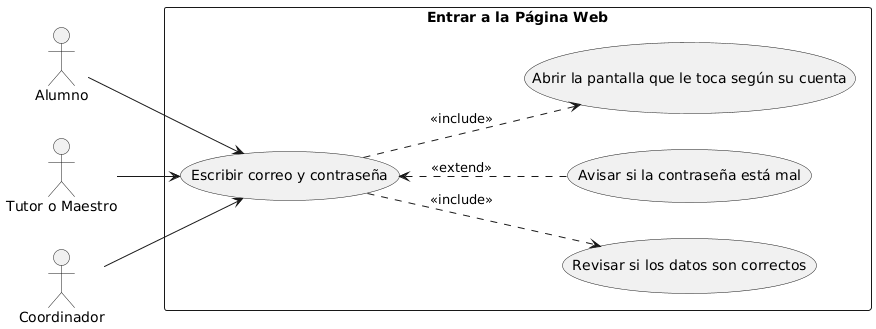
\includegraphics[width=0.88\textwidth]{assets/casos_uso/cu01_login.png}
    \caption{Diagrama del Caso de Uso 1: Iniciar Sesión en la Página Web.}
    \label{fig:cu01_login}
\end{figure}

% ----------------------------------------------------------------------
% CASO DE USO 2: REVISIÓN Y ENTREGA DE BORRADORES
% ----------------------------------------------------------------------
\subsection{Caso de Uso 2: Subir y Revisar Borradores de Tesis en PDF (CU02)}
\label{subsec:cu02}

En esta parte se muestra el camino para que el alumno entregue sus archivos de tesis, el maestro los pueda descargar para leerlos y dejar comentarios con correcciones, y la coordinación pueda ver que el trabajo siga avanzando sin perder copias viejas.

\begin{small}
\begin{longtable}{p{3.5cm} p{11.5cm}}
\caption{Descripción del Caso de Uso 2: Subida y revisión de tesis.} \label{tab:cu02} \\
\toprule
\textbf{Elemento} & \textbf{Detalle descriptivo} \\
\midrule
\endfirsthead

\multicolumn{2}{c}{\tablename\ \thetable\ -- Continuación de la página anterior} \\
\toprule
\textbf{Elemento} & \textbf{Detalle descriptivo} \\
\midrule
\endhead

\bottomrule
\endfoot

\bottomrule
\endlastfoot

\textbf{Identificador} & CU02 \\ \addlinespace
\textbf{Nombre} & Manejo y entrega de borradores de tesis \\ \addlinespace
\textbf{Participantes} & Alumno (sube el trabajo), Tutor o Maestro (descarga y revisa), Coordinador (revisa el avance general). \\ \addlinespace
\textbf{Propósito} & Guardar ordenadamente los archivos de la tesis para conservar la historia completa de cambios. \\ \addlinespace
\textbf{Requisitos previos} & Que el alumno tenga una cuenta activa y un maestro asignado en la página web. \\ \addlinespace
\textbf{Pasos principales} & 
1. El alumno entra a su apartado de entregas dentro de la página web.\par
2. Elige el archivo en su computadora, escribe una nota opcional y presiona ``Subir borrador''.\par
3. La página web revisa el archivo y le asigna un número de versión para ordenarlo (Versión 1, Versión 2, etc.).\par
4. El maestro entra a la página web y ve que su alumno subió un trabajo nuevo.\par
5. El maestro presiona el archivo para descargarlo y leerlo con calma.\par
6. En esa misma pantalla, el maestro anota sus observaciones o correcciones y las guarda.\par
7. Tanto el alumno como la coordinación pueden revisar la lista de entregas pasadas y los comentarios del maestro. \\ \addlinespace
\textbf{Caminos alternativos} & Si el estudiante intenta subir un archivo en un formato que no sea PDF (como Word o fotos), la página web lo rechaza y le pide elegir un documento en PDF. \\ \addlinespace
\textbf{Reglas obligatorias} & 
1. \textbf{Solo formato PDF:} Únicamente se aceptan archivos PDF para asegurar que las letras, tablas e imágenes no se muevan de lugar al abrirlos en otra computadora \parencite{iso32000}.\par
2. \textbf{No borrar archivos viejos:} La página web prohíbe eliminar o sobreescribir trabajos anteriores; cada entrega se guarda aparte para no perder ninguna corrección \parencite{chacon2014progit}. \\
\end{longtable}
\end{small}

En la Figura~\ref{fig:cu02_avances} se muestra el diagrama con las acciones de este apartado, donde se ve cómo el alumno sube el documento y el maestro lo descarga para responderle con sus observaciones.

\begin{figure}[H]
    \centering
    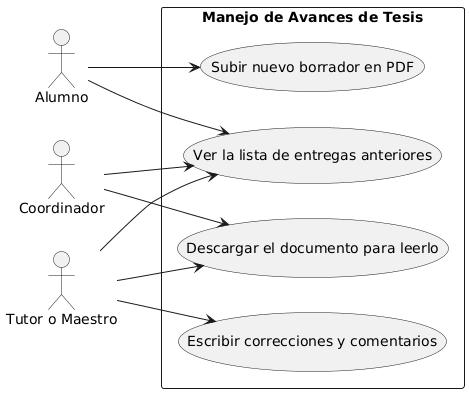
\includegraphics[width=0.72\textwidth]{assets/casos_uso/cu02_avances.png}
    \caption{Diagrama del Caso de Uso 2: Manejo de Avances de Tesis.}
    \label{fig:cu02_avances}
\end{figure}

% ----------------------------------------------------------------------
% CASO DE USO 3: REGISTRO DE MINUTAS
% ----------------------------------------------------------------------
\subsection{Caso de Uso 3: Llenar y Consultar Minutas de Asesoría (CU03)}
\label{subsec:cu03}

Aquí se explica la forma en que se guardan los acuerdos por escrito cada vez que el maestro y el alumno se juntan a revisar la tesis, evitando que las tareas se olviden con los días.

\begin{small}
\begin{longtable}{p{3.5cm} p{11.5cm}}
\caption{Descripción del Caso de Uso 3: Minutas de asesoría.} \label{tab:cu03} \\
\toprule
\textbf{Elemento} & \textbf{Detalle descriptivo} \\
\midrule
\endfirsthead

\multicolumn{2}{c}{\tablename\ \thetable\ -- Continuación de la página anterior} \\
\toprule
\textbf{Elemento} & \textbf{Detalle descriptivo} \\
\midrule
\endhead

\bottomrule
\endfoot

\bottomrule
\endlastfoot

\textbf{Identificador} & CU03 \\ \addlinespace
\textbf{Nombre} & Llenar y consultar minutas de asesoría \\ \addlinespace
\textbf{Participantes} & Tutor o Maestro (escribe la minuta), Alumno (revisa sus tareas), Coordinador (supervisa las reuniones). \\ \addlinespace
\textbf{Propósito} & Dejar un registro claro de lo que se habló en la reunión y qué tareas debe entregar cada quien para la siguiente cita. \\ \addlinespace
\textbf{Requisitos previos} & Haber terminado una reunión de asesoría (ya sea en persona o por videollamada). \\ \addlinespace
\textbf{Pasos principales} & 
1. Al terminar la reunión, el maestro entra a la sección de minutas en la página web.\par
2. Presiona el botón que dice ``Nueva minuta''.\par
3. Anota la fecha del día y un resumen corto de los temas de los que hablaron.\par
4. En la parte de compromisos, escribe las tareas pendientes, quién las va a hacer (el alumno o el maestro) y para qué fecha deben estar listas.\par
5. Presiona el botón de guardar.\par
6. La página web guarda los datos al instante.\par
7. El alumno puede entrar en cualquier momento a consultar qué tareas tiene pendientes y cuándo entregarlas. \\ \addlinespace
\textbf{Caminos alternativos} & Si el maestro intenta guardar la minuta dejando espacios en blanco o sin anotar compromisos, la página web no lo deja guardar y le avisa qué datos le faltan. \\ \addlinespace
\textbf{Regla obligatoria} & \textbf{Datos obligatorios:} Toda minuta debe llevar forzosamente la fecha de la reunión, de qué hablaron y por lo menos una tarea con fecha límite de entrega. \\
\end{longtable}
\end{small}

Para entender el proceso de forma visual, en la Figura~\ref{fig:cu03_minutas} se representa el diagrama de cómo el maestro anota los acuerdos y cómo los demás usuarios pueden consultar esa información.

\begin{figure}[H]
    \centering
    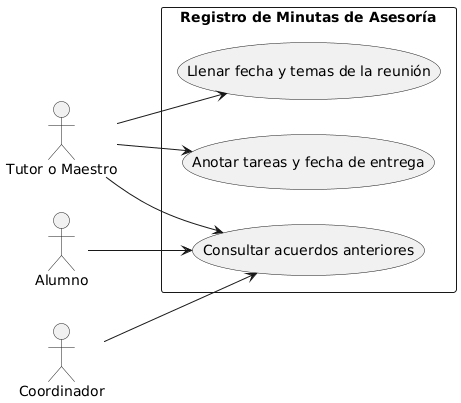
\includegraphics[width=0.68\textwidth]{assets/casos_uso/cu03_minutas.png}
    \caption{Diagrama del Caso de Uso 3: Registro de Minutas de Asesoría.}
    \label{fig:cu03_minutas}
\end{figure}

% ----------------------------------------------------------------------
% CASO DE USO 4: ALERTAS DE INACTIVIDAD
% ----------------------------------------------------------------------
\subsection{Caso de Uso 4: Avisos por Inactividad Mayor a 30 Días (CU04)}
\label{subsec:cu04}

Este caso de uso describe la función que hace la página web de contar los días sin actividad para avisar a los maestros y a la coordinación cuando un estudiante se está quedando atrás y necesita apoyo.

\begin{small}
\begin{longtable}{p{3.5cm} p{11.5cm}}
\caption{Descripción del Caso de Uso 4: Avisos de inactividad.} \label{tab:cu04} \\
\toprule
\textbf{Elemento} & \textbf{Detalle descriptivo} \\
\midrule
\endfirsthead

\multicolumn{2}{c}{\tablename\ \thetable\ -- Continuación de la página anterior} \\
\toprule
\textbf{Elemento} & \textbf{Detalle descriptivo} \\
\midrule
\endhead

\bottomrule
\endfoot

\bottomrule
\endlastfoot

\textbf{Identificador} & CU04 \\ \addlinespace
\textbf{Nombre} & Detección y aviso de inactividad mayor a 30 días \\ \addlinespace
\textbf{Participantes} & Página Web (reloj automático), Tutor o Maestro (cuida a sus alumnos), Coordinador (revisa a todos los alumnos). \\ \addlinespace
\textbf{Propósito} & Avisar a tiempo si un alumno lleva mucho tiempo sin comunicarse o sin entregar avances, para ayudarlo antes de que deje la tesis \parencite{lando2025digital}. \\ \addlinespace
\textbf{Requisitos previos} & Que los alumnos estén registrados y tengan la fecha de su último trabajo o de su última reunión. \\ \addlinespace
\textbf{Pasos principales} & 
1. La página web compara la fecha de hoy con el último día en que el estudiante subió un archivo o tuvo una reunión.\par
2. La página web cuenta cuántos días han pasado sin registrar nada nuevo.\par
3. Si la cuenta pasa de los 30 días, la página web le pone una marca de alerta al expediente del estudiante.\par
4. Cuando el maestro abre su lista de tesistas, ve un aviso junto al nombre del alumno atrasado.\par
5. Cuando el coordinador abre su pantalla, ve una lista con todos los alumnos que tienen alerta para llamarlos o mandarles un mensaje a tiempo. \\ \addlinespace
\textbf{Caminos alternativos} & En cuanto el alumno vuelve a subir un trabajo en PDF o el maestro registra una nueva minuta, el contador de días se regresa a cero y el aviso de alerta se apaga automáticamente. \\ \addlinespace
\textbf{Regla obligatoria} & \textbf{Tiempo límite de 30 días:} El aviso se enciende únicamente cuando el alumno acumula más de 30 días seguidos sin entregar ningún trabajo y sin registrar minutas de asesoría. \\
\end{longtable}
\end{small}

De forma gráfica, en la Figura~\ref{fig:cu04_atrasos} se muestra cómo el reloj de la página web cuenta los días y activa la lista de alertas para que los maestros y la coordinación puedan intervenir a tiempo.

\begin{figure}[H]
    \centering
    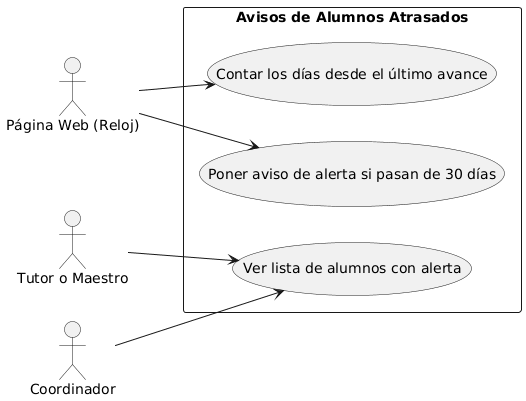
\includegraphics[width=0.68\textwidth]{assets/casos_uso/cu04_atrasos.png}
    \caption{Diagrama del Caso de Uso 4: Avisos de Alumnos Atrasados.}
    \label{fig:cu04_atrasos}
\end{figure}
\section{Diseño de la Base de Datos}
\label{sec:diseno_bd}

En este apartado se explica cómo se guarda y se organiza la información dentro de la página web usando una base de datos relacional \parencite{silberschatz2014}. Toda la información se reparte en tablas conectadas entre sí para que nada se pierda ni se revuelva, asegurando que las cuentas funcionen bien, los archivos en PDF se guarden por versiones sin borrar nada viejo, las reuniones queden registradas con sus tareas y el sistema avise si alguien pasa más de un mes sin trabajar \parencite{sim2023technology}.

\subsection{Descripción del Proyecto y Elementos de la Base de Datos}
\label{subsec:descripcion_bd}

Para entender el diagrama del sistema, la información se organiza en tres cosas muy sencillas: las tablas principales que representan a los elementos del sistema (rectángulos), los datos específicos que guarda cada una (óvalos o bolitas) y las conexiones que explican cómo se relacionan entre sí (rombos) \parencite{silberschatz2014}.

\subsubsection{Tablas y qué datos guarda cada una}

La base de datos empieza con la tabla llamada \textit{usuario}, que sirve para controlar el acceso de todas las personas a la página web. Esta tabla utiliza como dato principal el \underline{id\_usuario}, que es un número único para cada cuenta que no se repite. Además, guarda datos básicos como el \textit{correo\_institucional} para iniciar sesión, la \textit{contrasena}, la \textit{fecha\_registro} y la casilla de \textit{cuenta\_activa} para saber si la persona puede entrar o está dada de baja. El nombre de la persona se guarda en un dato llamado \textit{nombre\_completo}, el cual se divide en primer nombre, segundo nombre, apellido paterno y apellido materno para que sea fácil ordenar las listas por orden alfabético. También incluye el dato de \textit{telefono}, que se dibuja con doble óvalo porque una persona puede registrar más de un número para que la localicen. Como no todos hacen lo mismo en la página web, esta cuenta general se divide en tres tipos de usuario: el \textit{alumno}, que guarda su matrícula escolar; el \textit{asesor}, que guarda su número de maestro y su grado de estudios; y el \textit{coordinador}, que guarda el número de su oficina y su teléfono de atención.

La siguiente tabla es \textit{proyecto\_tesis}, que funciona como el expediente principal del trabajo de investigación. Tiene su propio identificador llamado \underline{id\_proyecto} y guarda datos como el \textit{titulo\_tesis}, el tema o \textit{linea\_investigacion}, la \textit{fecha\_inicio}, la \textit{fecha\_ultimo\_avance} y cómo va el trabajo en el \textit{estado\_proyecto}. En esta tabla se incluye un dato especial llamado \textit{dias\_inactividad}, que en el dibujo lleva una bolita con línea punteada porque nadie lo escribe a mano; la página web hace una resta automática entre la fecha de hoy y la fecha del último avance para saber cuántos días lleva el alumno sin entregar nada.

Para guardar los documentos del estudiante se utiliza la tabla \textit{entregable\_version}. En el dibujo se coloca con un rectángulo doble porque es una tabla dependiente; es decir, no tiene sentido guardar un archivo suelto si no pertenece a una tesis ya registrada. Esta tabla usa el dato \underline{numero\_version} para enumerar las entregas (como versión 1, versión 2 o versión 3), logrando que cada trabajo nuevo se guarde por separado sin borrar los archivos anteriores. También guarda la \textit{ruta\_archivo\_pdf} donde quedó el documento, la \textit{fecha\_hora\_subida}, una nota escrita por el estudiante en \textit{comentario\_alumno} y las correcciones que le escribe el maestro en \textit{retroalimentacion\_asesor}.

Para llevar el control de las citas de asesoría se tiene la tabla \textit{minutas\_asesoria}, que se identifica con el número \underline{id\_minuta}. Aquí se guarda la \textit{fecha\_reunion}, si la cita fue en persona o por internet en \textit{modalidad}, un resumen de lo que platicaron en \textit{resumen\_temas} y el día en que se capturó la información en \textit{fecha\_registro}.

Pegada a cada minuta se encuentra la tabla \textit{compromiso\_acuerdo}, que también se dibuja con recuadro doble porque las tareas solo existen si se acordaron en una reunión previa. Se organiza mediante el número de tarea \underline{numero\_acuerdo} y guarda qué hay que hacer en \textit{descripcion\_tarea}, a quién le toca cumplirla en \textit{responsable} (si al alumno o al maestro), el día máximo de entrega en \textit{fecha\_limite} y una casilla de \textit{estado\_cumplido} para marcar si ya se entregó o si sigue pendiente.

Por último, se encuentra la tabla \textit{alerta\_rezago}, que se encarga de guardar los avisos automáticos que manda la página web. Cuenta con su número de aviso \underline{id\_alerta} y guarda el día del aviso en \textit{fecha\_deteccion}, cuántos días sin avance se contaron en \textit{dias\_acumulados} y si el aviso ya fue atendido por el profesor en \textit{estado\_alerta}.

\subsubsection{Cómo se conectan las tablas y cuántos datos abarcan (Cardinalidades)}

Las líneas y los rombos del dibujo muestran cómo se comunica una tabla con otra y cuántos registros puede tener cada conexión. La tabla general de \textit{usuario} se conecta con cada tipo de cuenta (\textit{alumno}, \textit{asesor} y \textit{coordinador}) mediante una relación de uno a uno ($1:1$), lo que significa que cada cuenta de la página web le pertenece exactamente a una sola persona con su perfil correspondiente.

A partir de ahí, el \textit{alumno} se une con \textit{proyecto\_tesis} mediante la acción Desarrolla con una relación de uno a uno ($1:1$). Esto indica que un estudiante solo puede tener una tesis activa en la página web y que cada tesis le pertenece a un solo alumno. En cambio, el \textit{asesor} se conecta con \textit{proyecto\_tesis} con la acción Dirige en una relación de uno a muchos ($1:N$), porque un profesor puede asesorar a varios alumnos al mismo tiempo, pero cada trabajo de tesis tiene a un solo maestro titular a cargo. Por su parte, el \textit{coordinador} se conecta con la tesis mediante la acción Supervisa ($1:N$), ya que la coordinación tiene permiso de entrar a revisar todos los proyectos registrados en la escuela sin ser el director directo de ninguno de ellos.

En cuanto al manejo de los trabajos y documentos, la tabla \textit{proyecto\_tesis} se conecta con \textit{entregable\_version} a través del rombo doble Guarda versiones ($1:N$). Esto significa que a lo largo de los meses una tesis va juntando muchos borradores en PDF, pero cada archivo pertenece estrictamente a ese trabajo. De la misma forma, el proyecto se conecta con \textit{minutas\_asesoria} mediante la acción Registra ($1:N$), acumulando todas las juntas que se realicen durante el posgrado. Cada minuta se conecta a su vez con la tabla dependiente \textit{compromiso\_acuerdo} mediante el rombo doble Contiene tareas ($1:N$), lo que asegura que de cada reunión salgan una o varias tareas obligatorias por cumplir. Para terminar, la tesis se conecta con \textit{alerta\_rezago} con la acción Dispara aviso ($1:N$), lo que permite que el sistema guarde una alerta cada vez que el reloj automático note que el estudiante lleva más de 30 días seguidos sin registrar avances ni minutas.

\clearpage

\subsection{Diagrama Entidad--Relación}
\label{subsec:diagrama_eer}

En la Figura~\ref{fig:diagrama_eer} se muestra el dibujo completo de la base de datos, donde se aprecian las tablas normales, las tablas dependientes con doble línea, los datos con sus diferentes tipos de bolitas y los números que indican cómo se unen entre sí.

\begin{figure}[htbp]
    \centering
    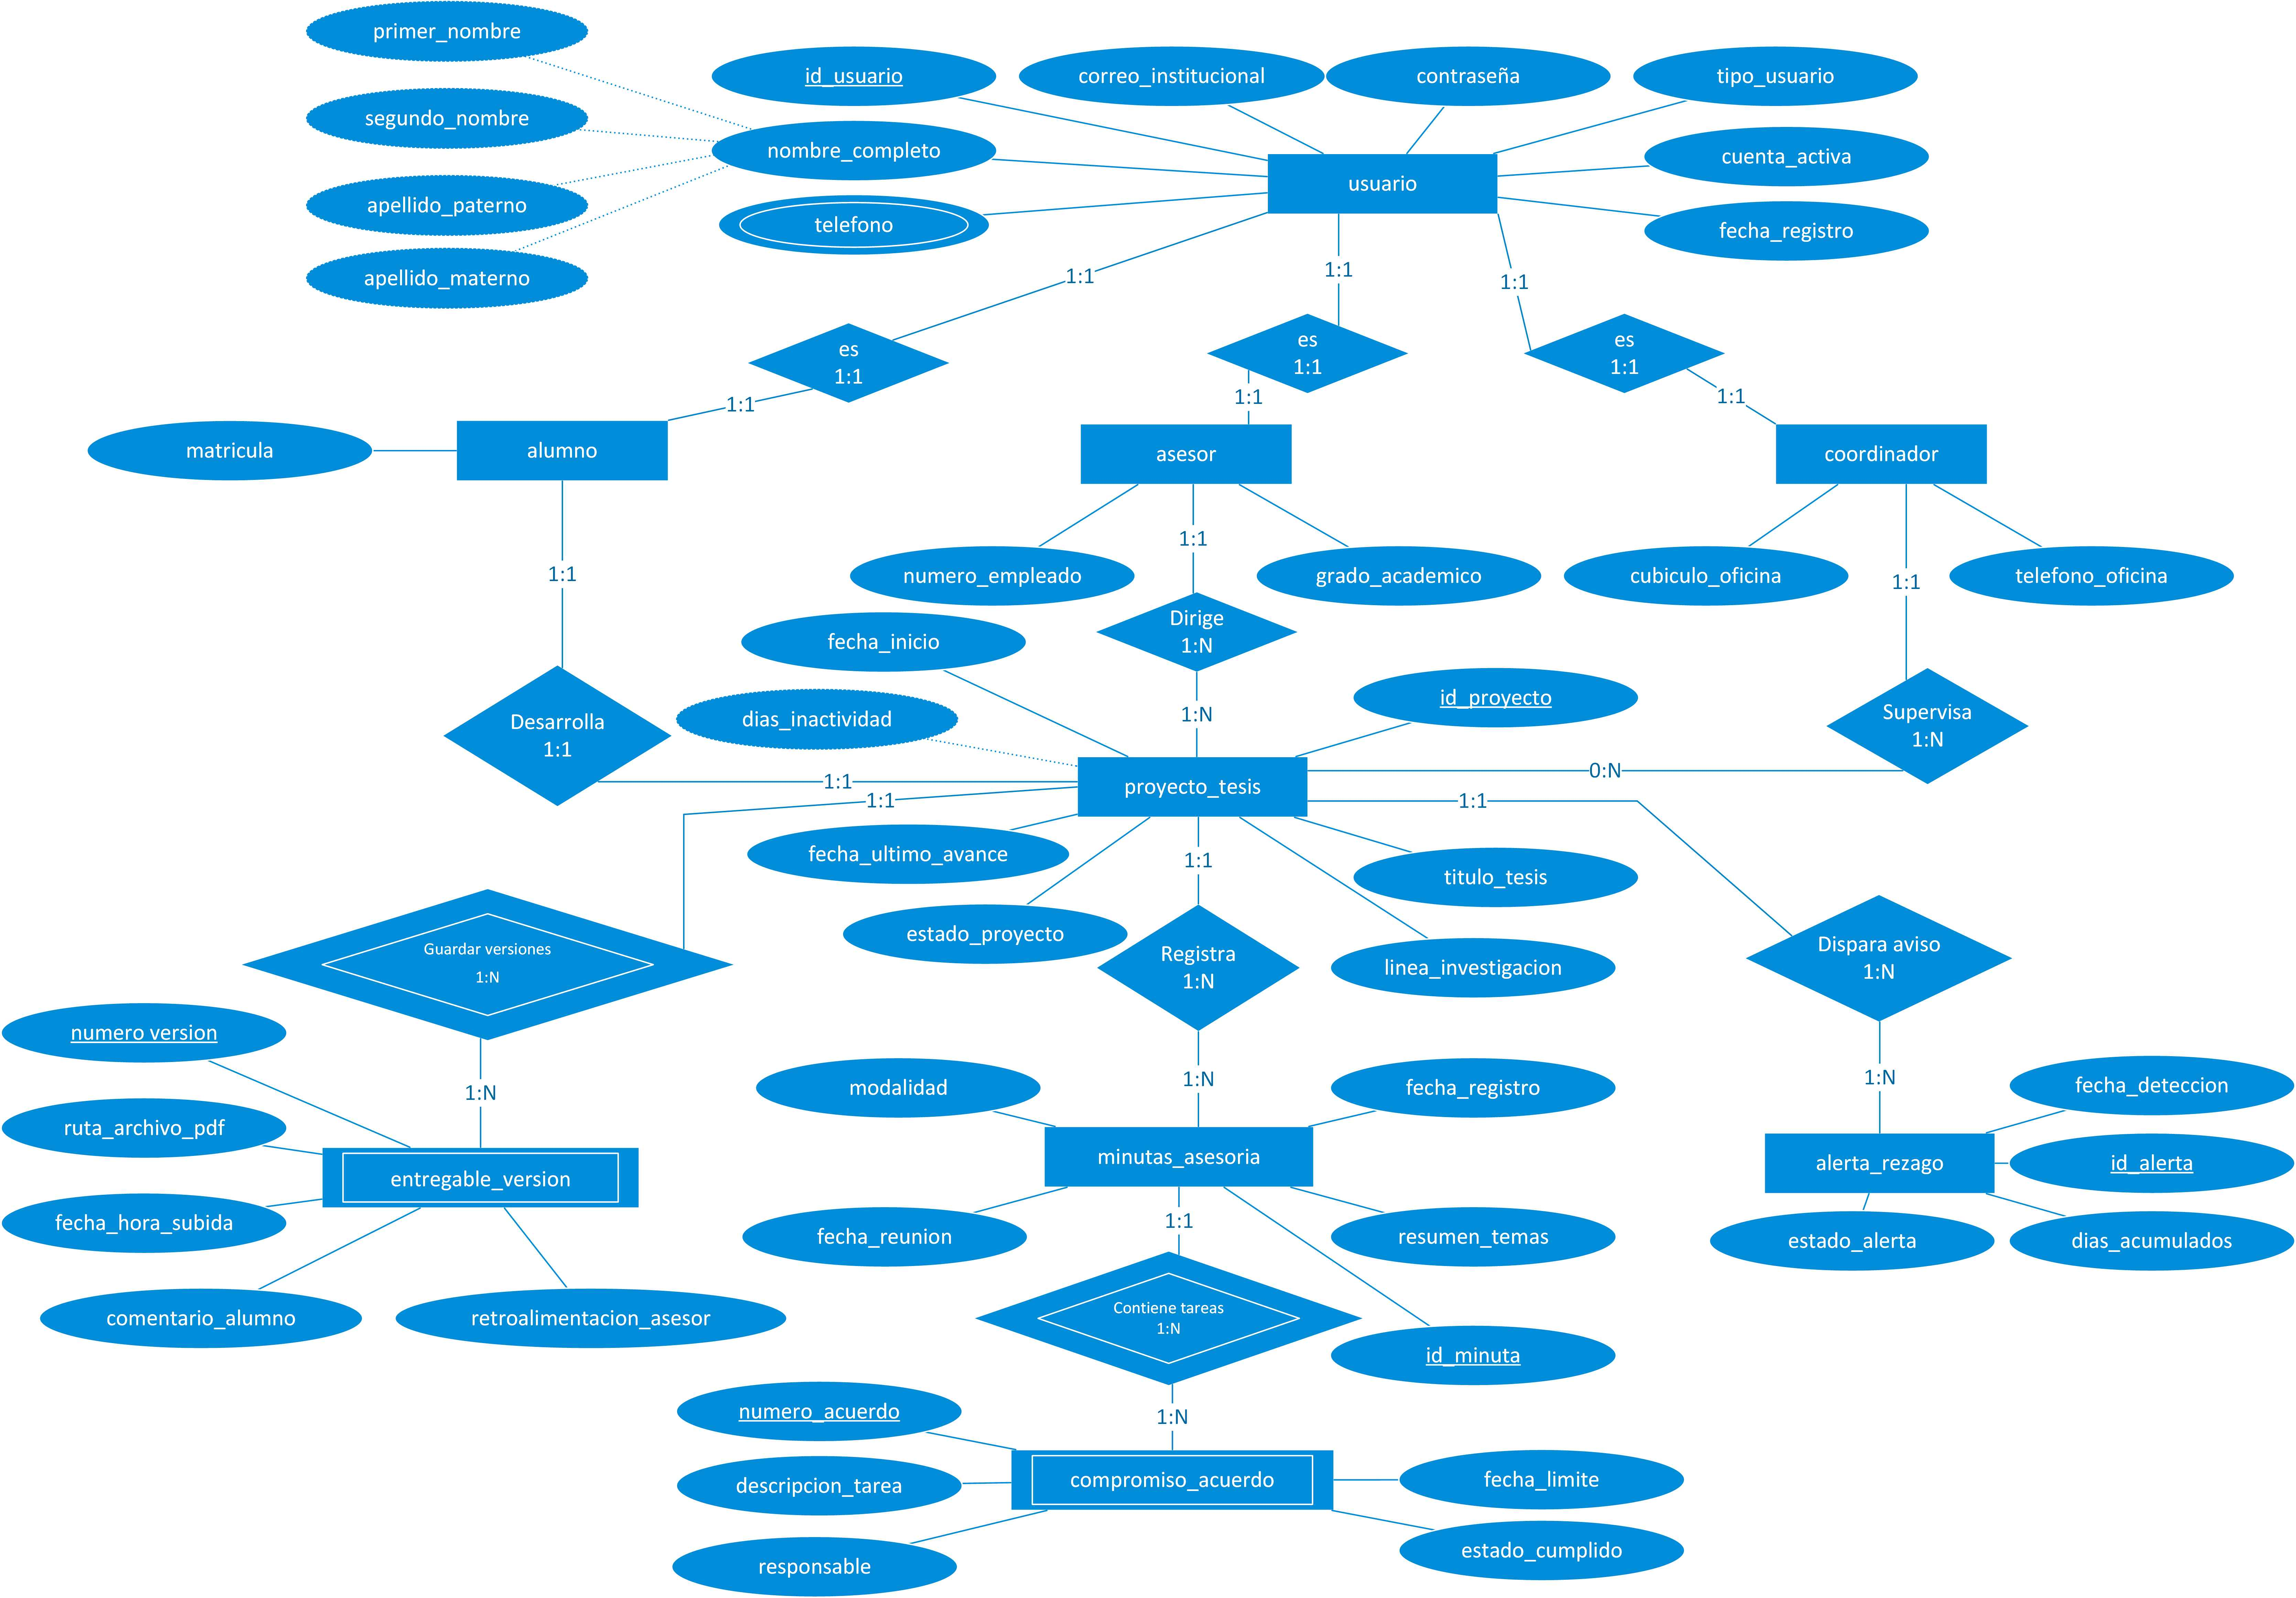
\includegraphics[width=1\linewidth]{assets/database/db-MER.jpg}
    \caption{Diagrama Entidad--Relación Extendido de la página web para seguimiento de tesis.}
    \label{fig:diagrama_eer}
\end{figure}

% ======================================================================
% BIBLIOGRAFÍA EN FORMATO APA 7
% ======================================================================
\nocite{*} 
\printbibliography[heading=bibintoc, title={Bibliografía}]

\end{document}